  \subsection{Ejercicio 8}

  A continuaci\'on se muestran los gr\'aficos del lote 8 ejecutado sobre los schedulers Round-Robin con y sin migraci\'on entre procesos.

  \begin{figure}
  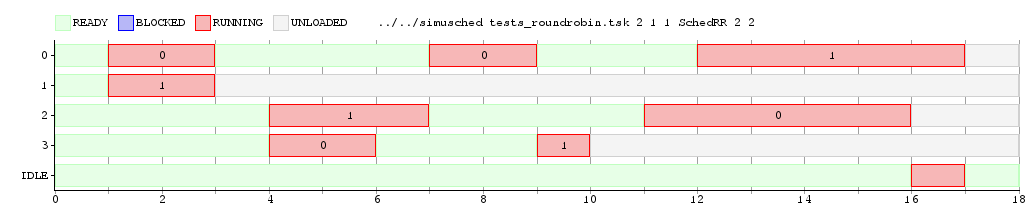
\includegraphics[scale=0.32]{images/ej8_RR.png}
  \caption{Diagrama de Gantt para el lote 8 en RR con dos n\'ucleos}
  \end{figure}

  \begin{figure}
  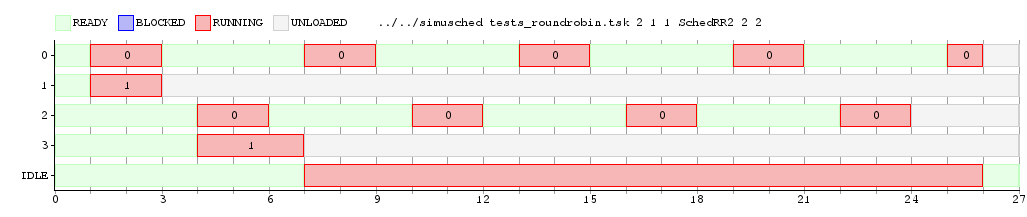
\includegraphics[scale=0.32]{images/ej8_RR2.png}
  \caption{Diagrama de Gantt para el lote 8 en RR2 con dos n\'ucleos}
  \end{figure}

  Se puede observar en el caso donde hay tareas con considerable diferencia de duracion, una mejor performance del scheduler RR1, dado que realiza una correccion permanente del balanceo de carga usando los recursos que tiene a su alcance en cada tick. Mientras que en el RR2, al quedar fija la afinidad al momento del dispatch, si ocurre un caso donde ambas tareas cortas quedan en un core y las tareas largas en otro core, al finalizar las tareas cortas, se desperdiciara un core durante toda la ejecucion de las tareas largas.
  Esta diferencia se ve claramente en los gr\'aficos 8 y 9 si notamos que cuando se usa RR1 se termina de ejecutar a tiempo 18 y con RR2 a tiempo 27, lo que es una diferencia abismal. Cabe destacar que para que esto pase se necesita
  que haya una gran diferencia entre el uso de CPU de las tareas y que las largas se encuentren concentradas en un n\'ucleo mientras las cortas en otro, lo que no suele ser un caso promedio.
